\documentclass[12pt, twoside]{article}
\usepackage[letterpaper, margin=1in, headsep=0.5in]{geometry}
\usepackage[english]{babel}
\usepackage[utf8]{inputenc}
\usepackage{amsmath}
\usepackage{amsfonts}
\usepackage{amssymb}
\usepackage{tikz}
\usetikzlibrary{quotes, angles}
\usepackage{graphicx}
%\usepackage{pgfplots}
%\pgfplotsset{width=10cm,compat=1.9}
%\usepgfplotslibrary{statistics}
%\usepackage{pgfplotstable}
%\usepackage{tkz-fct}
%\usepackage{venndiagram}
\usepackage{multicol}


\usepackage{fancyhdr}
\pagestyle{fancy}
\fancyhf{}
\fancyhead[LE]{\thepage}
\fancyhead[RO]{\thepage \\Name: \hspace{4cm} \,\\}
\fancyhead[LO]{BECA / Dr. Huson / Geometry 10th Grade\\* Unit 9: Congruence transformations \\ 26 February 2020}

\renewcommand{\headrulewidth}{0pt}

\begin{document}
\subsubsection*{9.3 Classwork: Triangle congruence theorem applications}
  \begin{enumerate}

    \item 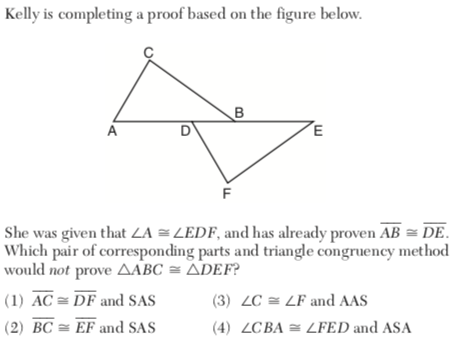
\includegraphics[scale=0.8]{geom-62017-9.png}
    \item Sketch the triangles first. \\
    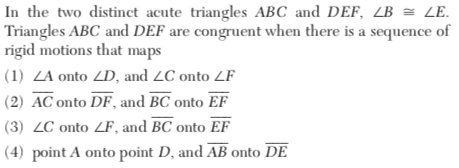
\includegraphics[scale=0.8]{geom-62017-22.png}
    \item Sketch the triangles first. \\
      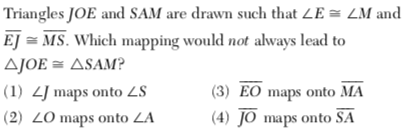
\includegraphics[scale=0.8]{geom-62019-14.png}
    \item 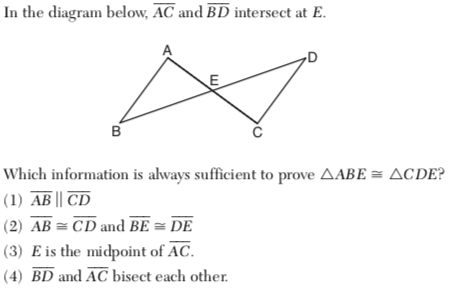
\includegraphics[scale=0.8]{geom-62019-8.png}
    \item Sketch the triangles first. \\
      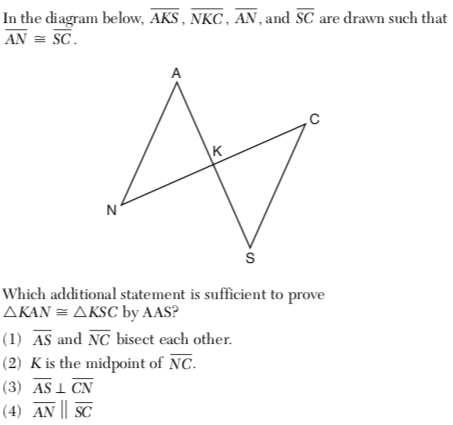
\includegraphics[scale=0.8]{geom-82019-10.png}

\end{enumerate}
\end{document}
